%=====================================================================
%  k8s-style.tex  --  Visual identity for "The Kubernetes Handbook"
%  Compile with pdfLaTeX (Overleaf default). Run twice for overlays.
%=====================================================================

%---------------------------------------------------------------------
% Encoding, fonts, page geometry
%---------------------------------------------------------------------
\usepackage[T1]{fontenc}
\usepackage[utf8]{inputenc}
\usepackage[sfdefault]{roboto}          % clean sans, close to the k8s.io look
\usepackage[scaled=0.84]{beramono}      % monospace with a real bold
\usepackage{microtype}
\usepackage[a4paper, top=2.6cm, bottom=2.6cm, left=2.3cm, right=2.3cm,
            headheight=20pt]{geometry}
\setlength{\parindent}{0pt}
\setlength{\parskip}{0.55em}
\linespread{1.08}

%---------------------------------------------------------------------
% Kubernetes colour palette
%---------------------------------------------------------------------
\usepackage[table,dvipsnames]{xcolor}
\definecolor{k8sblue}{HTML}{326CE5}     % official Kubernetes blue
\definecolor{k8sdeep}{HTML}{1D4AA8}
\definecolor{k8snavy}{HTML}{0F2A5C}
\definecolor{k8smid}{HTML}{8FB0F2}
\definecolor{k8slight}{HTML}{EAF1FD}
\definecolor{k8sgray}{HTML}{5F6B7A}
\definecolor{k8sorange}{HTML}{F5A623}
\definecolor{k8sgreen}{HTML}{2EAD6B}
\definecolor{k8sred}{HTML}{E2483D}
\definecolor{k8spurple}{HTML}{7B5CD6}
\definecolor{k8steal}{HTML}{14A3A3}
\definecolor{codebg}{HTML}{F6F8FC}
\definecolor{codetext}{HTML}{1F2933}
\definecolor{codecomment}{HTML}{7A8699}
\definecolor{codestring}{HTML}{1E8A55}

%---------------------------------------------------------------------
% Packages
%---------------------------------------------------------------------
\usepackage{graphicx}
\graphicspath{{images/}}
\usepackage{fontawesome5}
\usepackage{amsmath,amssymb}
\usepackage{array,booktabs,tabularx,multirow,longtable}
\usepackage{enumitem}
\usepackage{multicol}
\usepackage{etoolbox}
\usepackage{eso-pic}
\usepackage{fancyhdr}
\usepackage[fit]{truncate}
\usepackage{titlesec}
\usepackage{listings}
\usepackage{tikz}
\usetikzlibrary{shapes.geometric,shapes.misc,positioning,arrows.meta,
                calc,fit,backgrounds,shadows,decorations.pathreplacing}
\usepackage[most]{tcolorbox}
\tcbuselibrary{listings}

%---------------------------------------------------------------------
% Lists
%---------------------------------------------------------------------
\setlist{itemsep=0.25em, topsep=0.35em}
\setlist[itemize,1]{label={\color{k8sblue}\small\faCaretRight}}
\setlist[itemize,2]{label={\color{k8smid}\scriptsize\faCircle}}
\setlist[enumerate,1]{label={\color{k8sblue}\bfseries\arabic*.}}

%---------------------------------------------------------------------
% Images and icons (fall back to a Font Awesome cube if a file is missing)
%---------------------------------------------------------------------
\DeclareRobustCommand{\kimg}[2][1cm]{%
  \IfFileExists{images/#2.png}%
    {\includegraphics[height=#1]{images/#2.png}}%
    {\textcolor{k8sblue}{\faCube}}}
\DeclareRobustCommand{\kicon}[2][1.15em]{\raisebox{-0.28\height}{\kimg[#1]{#2}}}

% Inline code, file names, and keyboard-ish terms
\newcommand{\kc}[1]{\textcolor{k8sdeep}{\texttt{#1}}}
\newcommand{\kterm}[1]{\textbf{\textcolor{k8snavy}{#1}}}

%---------------------------------------------------------------------
% Tables
%---------------------------------------------------------------------
\newcolumntype{L}{>{\raggedright\arraybackslash}X}
\newcolumntype{P}[1]{>{\raggedright\arraybackslash}p{#1}}
\newcommand{\kth}[1]{\textcolor{white}{\bfseries #1}}
\newcommand{\ktablestart}{\rowcolors{2}{k8slight}{white}\renewcommand{\arraystretch}{1.35}}
\newcommand{\kheader}{\rowcolor{k8sblue}}

%---------------------------------------------------------------------
% Page header / footer
%---------------------------------------------------------------------
\pagestyle{fancy}
\fancyhf{}
\renewcommand{\chaptermark}[1]{\markboth{#1}{}}
\renewcommand{\sectionmark}[1]{\markright{\thesection\quad #1}}
\fancyhead[L]{\kicon[1.25em]{k8s-logo}\hspace{0.5em}\small\bfseries\color{k8snavy}\truncate{0.5\textwidth}{\leftmark}}
\fancyhead[R]{\small\color{k8sgray}\truncate{0.4\textwidth}{\rightmark}}
\fancyfoot[L]{\footnotesize\color{k8sgray}The Kubernetes Handbook}
\fancyfoot[R]{\colorbox{k8sblue}{\makebox[1.6em]{\textcolor{white}{\bfseries\small\thepage}}}}
\renewcommand{\headrule}{{\color{k8sblue}\hrule height 0.9pt}}
\renewcommand{\footrulewidth}{0pt}
\fancypagestyle{plain}{%
  \fancyhf{}%
  \fancyfoot[L]{\footnotesize\color{k8sgray}The Kubernetes Handbook}%
  \fancyfoot[R]{\colorbox{k8sblue}{\makebox[1.6em]{\textcolor{white}{\bfseries\small\thepage}}}}%
  \renewcommand{\headrulewidth}{0pt}}

%---------------------------------------------------------------------
% Chapter banners
%---------------------------------------------------------------------
\newlength{\kchapw}
\def\kchapicon{k8s-logo}
\newcommand{\kchapter}[2]{\gdef\kchapicon{#2}\chapter{#1}}

\newcommand{\kchaptertitle}[1]{%
  \setlength{\kchapw}{\linewidth}\addtolength{\kchapw}{-7.2cm}%
  \begin{tikzpicture}
    \fill[k8sblue, rounded corners=8pt] (0,0) rectangle (\linewidth,3.4cm);
    \fill[k8sorange] (3.35cm,0.45cm) rectangle (5.35cm,0.55cm);
    \node[regular polygon, regular polygon sides=7, fill=white,
          minimum size=2.5cm, inner sep=0pt] at (1.75cm,1.8cm)
          {\color{k8sblue}\fontsize{32}{32}\selectfont\bfseries\thechapter};
    \node[anchor=west, text width=\kchapw, align=left, text=white]
          at (3.35cm,1.8cm)
          {{\small\bfseries\color{k8slight}\MakeUppercase{\chaptername}\ \thechapter}\\[5pt]
           {\fontsize{22}{26}\selectfont\bfseries #1}};
    \node[fill=white, rounded corners=6pt, inner sep=5pt]
          at (\linewidth-1.75cm,1.8cm) {\kimg[1.9cm]{\kchapicon}};
  \end{tikzpicture}}

\newcommand{\kchaptertitlenn}[1]{%
  \begin{tikzpicture}
    \fill[k8sblue, rounded corners=8pt] (0,0) rectangle (\linewidth,2.2cm);
    \node[anchor=west, text=white] at (0.6cm,1.1cm)
         {\kimg[1.3cm]{k8s-logo-white}\hspace{0.7em}\fontsize{24}{28}\selectfont\bfseries #1};
  \end{tikzpicture}}

\titleformat{\chapter}[block]{\normalfont}{}{0pt}{\kchaptertitle}
\titleformat{name=\chapter,numberless}[block]{\normalfont}{}{0pt}{\kchaptertitlenn}
\titlespacing*{\chapter}{0pt}{-25pt}{28pt}

%---------------------------------------------------------------------
% Section styles
%---------------------------------------------------------------------
\titleformat{\section}[hang]
  {\normalfont\Large\bfseries\color{k8snavy}}
  {\colorbox{k8sblue}{\textcolor{white}{\thesection}}}{0.6em}{}
  [\vspace{1pt}{\color{k8sblue!35}\titlerule[0.8pt]}]
\titlespacing*{\section}{0pt}{1.6em}{0.9em}

\titleformat{\subsection}[hang]
  {\normalfont\large\bfseries\color{k8sblue}}
  {\thesubsection}{0.6em}{}
\titlespacing*{\subsection}{0pt}{1.2em}{0.5em}

\titleformat{\subsubsection}[hang]
  {\normalfont\normalsize\bfseries\color{k8sdeep}}
  {\faAngleDoubleRight}{0.4em}{}

%---------------------------------------------------------------------
% Part pages (navy background, white type)
%---------------------------------------------------------------------
\def\kpartsub{}
\newcommand{\kpartbackground}{%
  \AtPageLowerLeft{%
    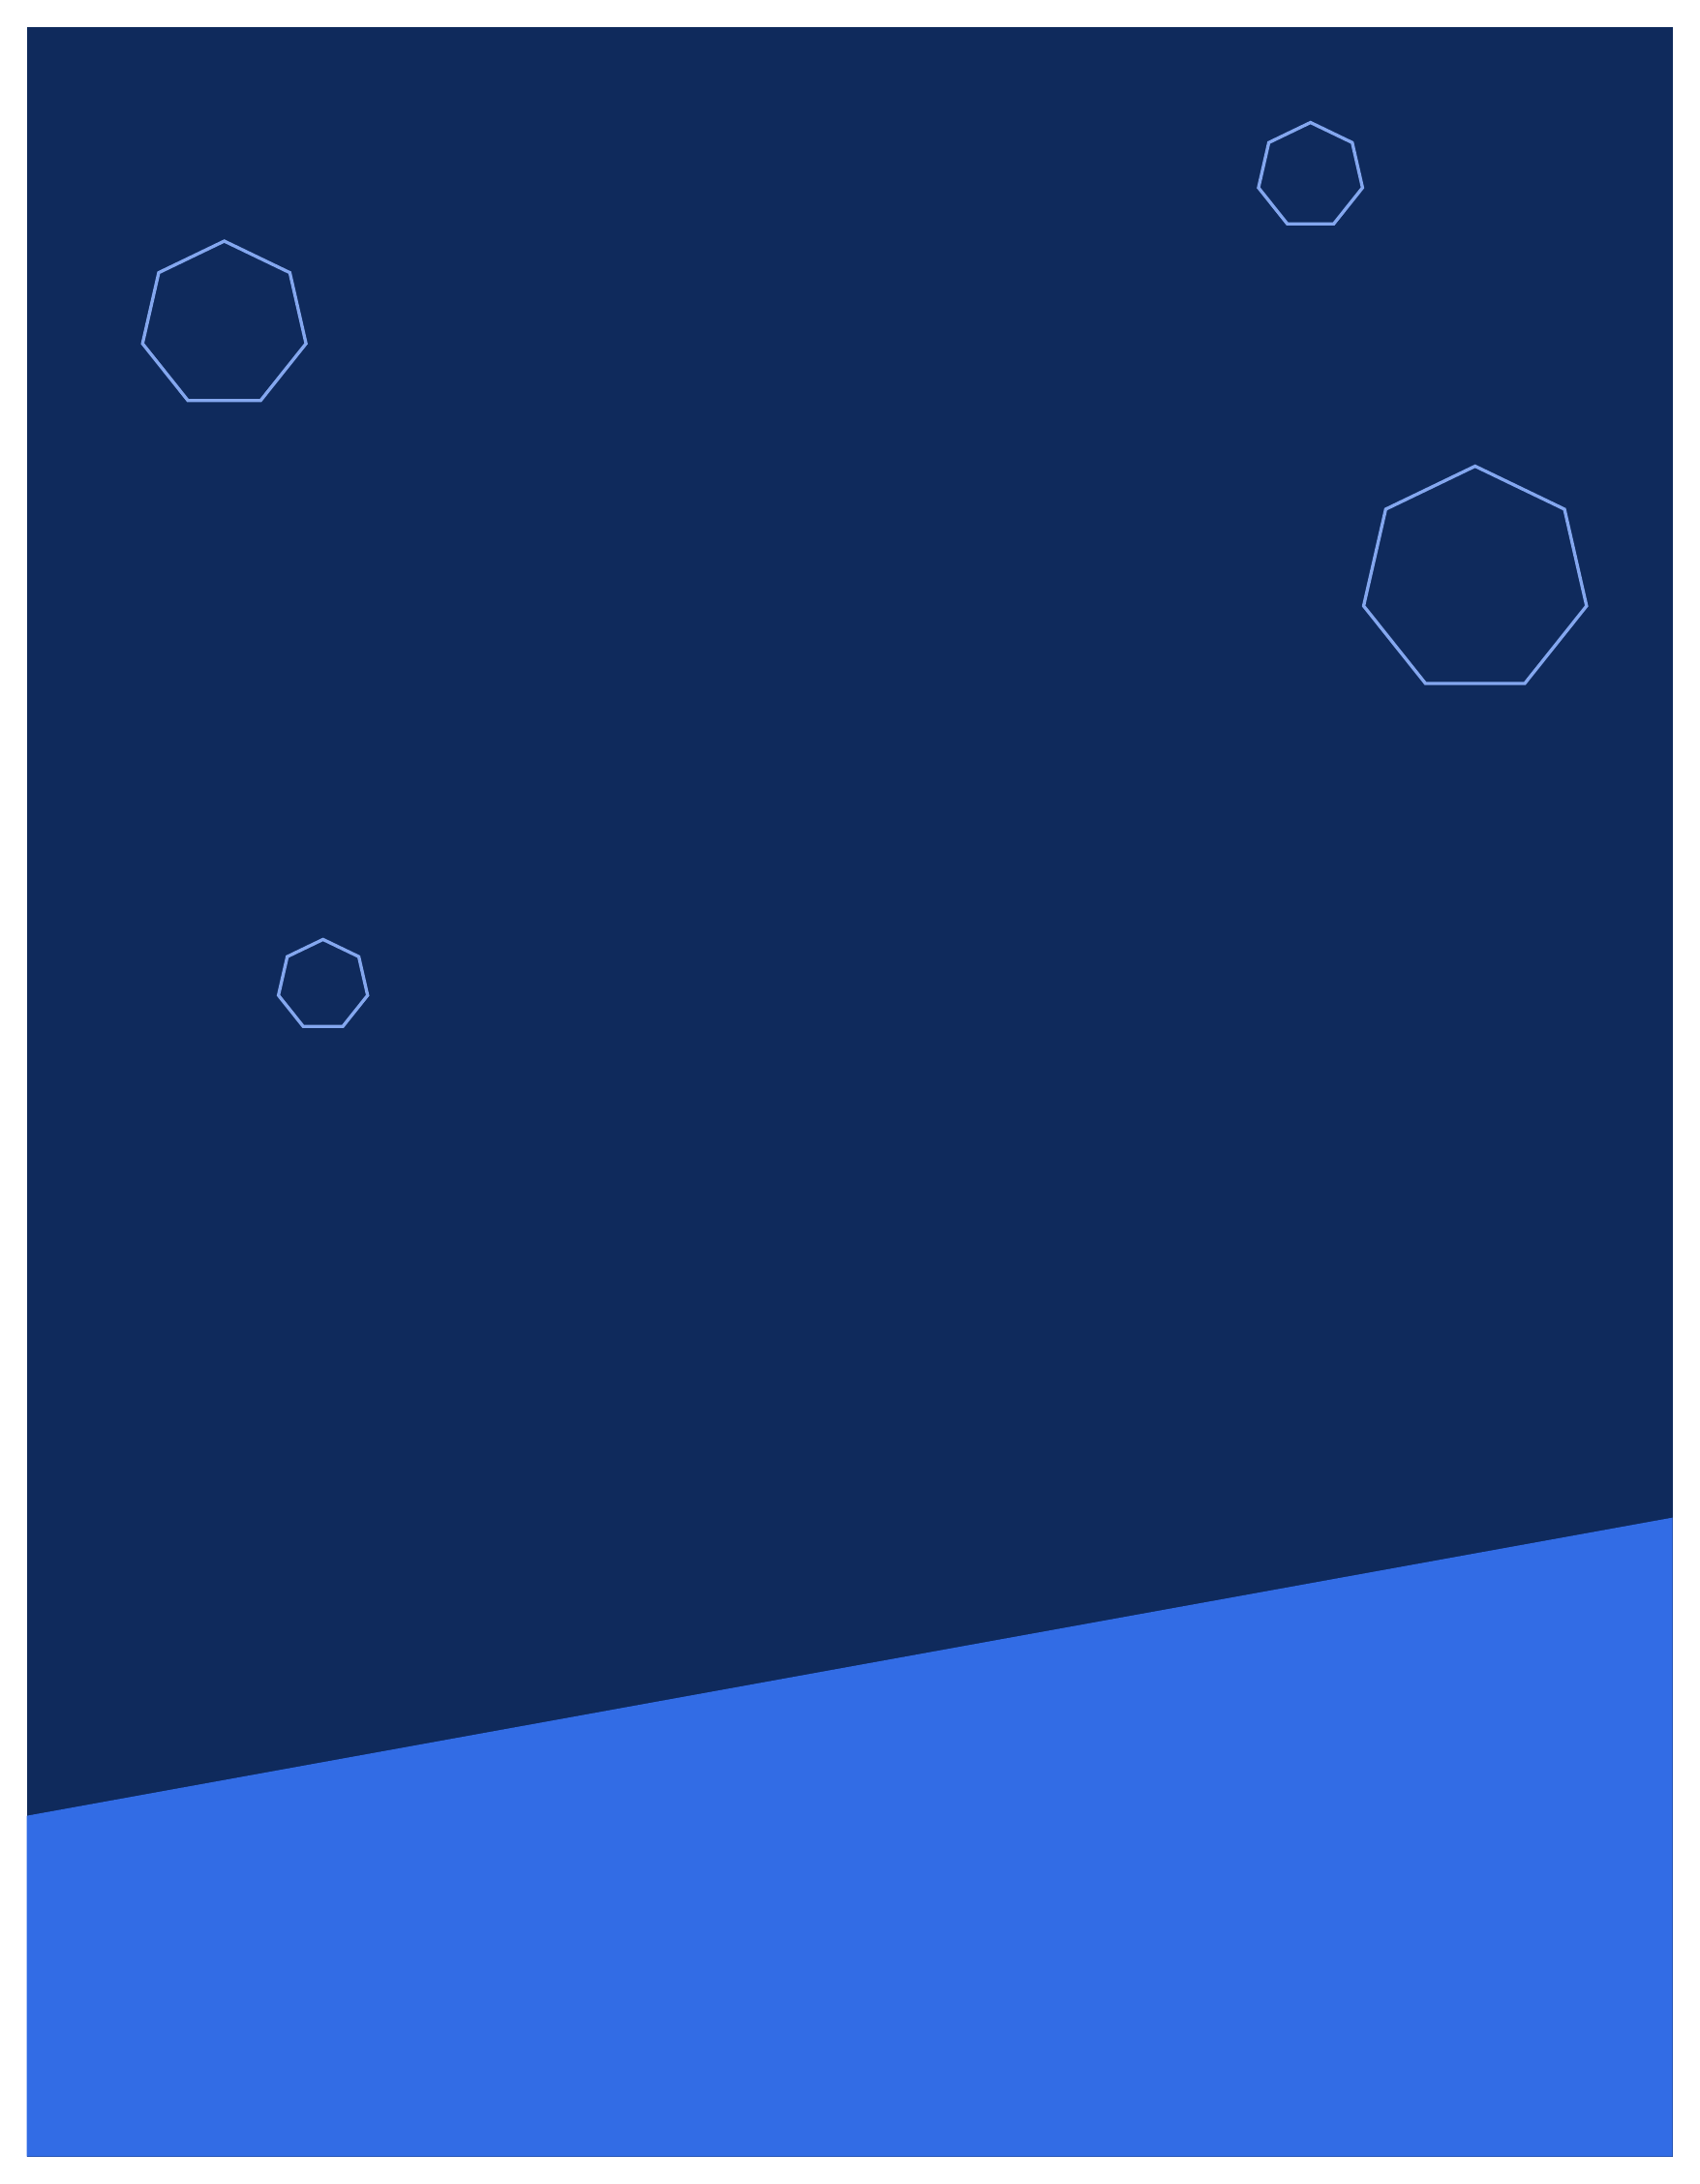
\begin{tikzpicture}
      \fill[k8snavy] (0,0) rectangle (\paperwidth,\paperheight);
      \fill[k8sblue] (0,0) -- (\paperwidth,0) -- (\paperwidth,0.30*\paperheight)
                     -- (0,0.16*\paperheight) -- cycle;
      \foreach \x/\y/\s in {0.12/0.86/2.2, 0.88/0.74/3.0, 0.78/0.93/1.4, 0.18/0.55/1.2}
        \node[regular polygon, regular polygon sides=7, draw=k8sblue!60,
              line width=1.2pt, minimum size=\s cm] at (\x*\paperwidth,\y*\paperheight) {};
    \end{tikzpicture}}}
\newcommand{\kpart}[2]{%
  \clearpage\gdef\kpartsub{#2}%
  \AddToShipoutPictureBG*{\kpartbackground}%
  \part{#1}}
\titleformat{\part}[display]
  {\centering\color{white}}
  {\kimg[3.6cm]{k8s-logo-white}\\[1.4em]{\large\bfseries\color{k8smid}PART \thepart}}
  {0.8em}
  {\fontsize{34}{42}\selectfont\bfseries}
  [\vspace{1.2em}{\large\itshape\color{k8slight}\kpartsub}]
\assignpagestyle{\part}{empty}

%---------------------------------------------------------------------
% Callout boxes
%---------------------------------------------------------------------
\tcbset{
  kbox/.style n args={3}{
    enhanced, breakable,
    colback=#1!6!white, colframe=#1, boxrule=0pt,
    leftrule=4pt, arc=3pt, outer arc=3pt,
    left=8pt, right=8pt, top=6pt, bottom=6pt,
    before skip=0.9em, after skip=0.9em,
    before upper={{\color{#1!80!black}\bfseries\small #2\hspace{0.45em}#3}\par\smallskip}
  }
}
\newtcolorbox{keyidea}[1][]{kbox={k8sblue}{\faKey}{Key Idea},#1}
\newtcolorbox{analogy}[1][]{kbox={k8steal}{\faLightbulb[regular]}{Real-World Analogy},#1}
\newtcolorbox{warningbox}[1][]{kbox={k8sred}{\faExclamationTriangle}{Watch Out},#1}
\newtcolorbox{tryit}[1][]{kbox={k8sgreen}{\faTerminal}{Try It Yourself},#1}
\newtcolorbox{protip}[1][]{kbox={k8spurple}{\faRocket}{Pro Tip},#1}
\newtcolorbox{deepdive}[1][]{kbox={k8sorange}{\faSearch}{Under the Hood},#1}

% Chapter recap box
\newtcolorbox{recap}[1][]{enhanced, breakable,
  colback=k8slight, colframe=k8sblue, boxrule=0.8pt, arc=4pt,
  title={\faCheckCircle\hspace{0.5em}Chapter Recap}, fonttitle=\bfseries,
  colbacktitle=k8sblue, coltitle=white, #1}

% "What you will learn" box at the start of each chapter
\newtcolorbox{objectives}[1][]{enhanced, breakable,
  colback=white, colframe=k8sblue!40, boxrule=0.6pt, arc=4pt,
  borderline west={4pt}{0pt}{k8sblue},
  title={\faMapSigns\hspace{0.5em}In this chapter you will learn}, fonttitle=\bfseries\small,
  colbacktitle=white, coltitle=k8sblue, #1}

%---------------------------------------------------------------------
% Code listings
%---------------------------------------------------------------------
\newcommand\YAMLcolonstyle{\color{k8snavy}\mdseries}
\newcommand\YAMLkeystyle{\color{k8sblue}\bfseries}
\newcommand\YAMLvaluestyle{\color{codetext}\mdseries}

\lstdefinelanguage{yaml}{
  keywords={true,false,null},
  keywordstyle=\color{k8sorange}\bfseries,
  sensitive=false,
  comment=[l]{\#},
  commentstyle=\color{codecomment}\itshape,
  stringstyle=\YAMLvaluestyle\color{codestring},
  moredelim=**[il][\YAMLcolonstyle{:}\YAMLvaluestyle]{:},
  morestring=[b]',
  morestring=[b]"
}

\lstdefinelanguage{docker}{
  keywords={FROM,AS,RUN,CMD,COPY,ADD,WORKDIR,ENV,EXPOSE,USER,ARG,LABEL,
            ENTRYPOINT,HEALTHCHECK,VOLUME,SHELL,ONBUILD,STOPSIGNAL},
  keywordstyle=\color{k8sblue}\bfseries,
  sensitive=true,
  comment=[l]{\#},
  commentstyle=\color{codecomment}\itshape,
  morestring=[b]",
  stringstyle=\color{codestring}
}

\lstset{
  basicstyle=\ttfamily\footnotesize\color{codetext},
  columns=fullflexible, keepspaces=true,
  showstringspaces=false, tabsize=2,
  breaklines=true, breakatwhitespace=false,
  postbreak=\mbox{\textcolor{k8sorange}{$\hookrightarrow$}\space},
  upquote=true,
  aboveskip=0pt, belowskip=0pt
}

\lstdefinestyle{kyaml}{language=yaml,
  basicstyle=\ttfamily\footnotesize\YAMLkeystyle}
\lstdefinestyle{kbash}{language=bash,
  keywordstyle=\color{k8sblue}\bfseries,
  morekeywords={kubectl,helm,docker,kind,minikube,k3d,git,curl,argocd,
                kustomize,sudo,brew,choco,winget,apt,make,base64,watch,
                openssl,jq,pip,python,pytest,trivy,velero,stern,k9s},
  commentstyle=\color{codecomment}\itshape,
  stringstyle=\color{codestring}}
\lstdefinestyle{kpython}{language=Python,
  keywordstyle=\color{k8sblue}\bfseries,
  commentstyle=\color{codecomment}\itshape,
  stringstyle=\color{codestring},
  morekeywords={async,await,with,as,self,None,True,False}}
\lstdefinestyle{kdocker}{language=docker}
\lstdefinestyle{khtml}{language=HTML,
  keywordstyle=\color{k8sblue}\bfseries,
  stringstyle=\color{codestring},
  commentstyle=\color{codecomment}\itshape,
  morekeywords={script,const,let,async,await,function,return,button,input,ul,li,main,section,header,meta,title,style}}
\lstdefinestyle{kplain}{language={}}

\tcbset{
  kcodebox/.style n args={2}{
    enhanced, breakable, listing only,
    colback=codebg, colframe=k8sblue!70, boxrule=0.6pt, arc=3pt,
    left=6pt, right=6pt, top=3pt, bottom=3pt,
    before skip=0.8em, after skip=0.9em,
    title={#1\hspace{0.5em}{\ttfamily\detokenize{#2}}},
    fonttitle=\footnotesize\bfseries, coltitle=white, colbacktitle=k8sblue,
    toptitle=1pt, bottomtitle=1pt
  }
}
\newtcblisting{yamlcode}[1]{kcodebox={\faFileCode[regular]}{#1}, listing options={style=kyaml}}
\newtcblisting{bashcode}[1]{kcodebox={\faTerminal}{#1}, listing options={style=kbash}}
\newtcblisting{pycode}[1]{kcodebox={\faPython}{#1}, listing options={style=kpython}}
\newtcblisting{dockercode}[1]{kcodebox={\faDocker}{#1}, listing options={style=kdocker}}
\newtcblisting{htmlcode}[1]{kcodebox={\faHtml5}{#1}, listing options={style=khtml}}
\newtcblisting{plaincode}[1]{kcodebox={\faFile[regular]}{#1}, listing options={style=kplain}}

%---------------------------------------------------------------------
% Hyperlinks (load last)
%---------------------------------------------------------------------
\usepackage[colorlinks=true, linkcolor=k8sdeep, urlcolor=k8sblue,
            citecolor=k8sblue, bookmarksnumbered=true,
            pdftitle={The Kubernetes Handbook},
            pdfauthor={The Kubernetes Handbook}]{hyperref}
\setcounter{tocdepth}{1}
\setcounter{secnumdepth}{2}
